\documentclass{ximera}

\usepackage{todonotes}

\newcommand{\RR}{\mathbb R}
\renewcommand{\d}{\,d}
\newcommand{\dd}[2][]{\frac{d #1}{d #2}}
\renewcommand{\l}{\ell}
\newcommand{\ddx}{\frac{d}{dx}}
\newcommand{\dfn}{\textbf}
\newcommand{\eval}[1]{\bigg[ #1 \bigg]}
\renewcommand{\epsilon}{\varepsilon}
\newcommand{\p}[1]{\left(#1\right)}
\newcommand{\br}[1]{\left[#1\right]}
\newcommand{\set}[1]{\left\{#1\right\}}


\let\prelim\lim
\renewcommand{\lim}{\displaystyle\prelim}

\colorlet{textColor}{black} 
\colorlet{background}{white}
\colorlet{penColor}{blue!50!black} % Color of a curve in a plot
\colorlet{penColor2}{red!50!black}% Color of a curve in a plot
\colorlet{penColor3}{red!50!blue} % Color of a curve in a plot
\colorlet{penColor4}{green!50!black} % Color of a curve in a plot
\colorlet{penColor5}{orange!80!black} % Color of a curve in a plot
\colorlet{fill1}{blue!50!black!20} % Color of fill in a plot
\colorlet{fill2}{blue!10} % Color of fill in a plot
\colorlet{fillp}{fill1} % Color of positive area
\colorlet{filln}{red!50!black!20} % Color of negative area
\colorlet{gridColor}{gray!50} % Color of grid in a plot


\newcommand{\fullwidth}{}
\newcommand{\normalwidth}{}



%% makes a snazzy t-chart for evaluating functions
\newenvironment{tchart}{\rowcolors{2}{}{background!90!textColor}\array}{\endarray}


\author{Gregory Hartman \and Matthew Carr}
\license{Creative Commons 3.0 By-NC}
\acknowledgement{https://github.com/APEXCalculus}

\begin{document}
\begin{exercise}

\outcome{Understand the derivative as a function related to the original function.}
\outcome{Relate the derivative function to the derivative at a point.}

%% BADBAD answer format? Does Ximera know that a=b iff b=a ? Does Ximera know that f'(x)=d/dx f(x) ?

Given the graph of both of the functions $g$ and $f$:

\begin{center}
 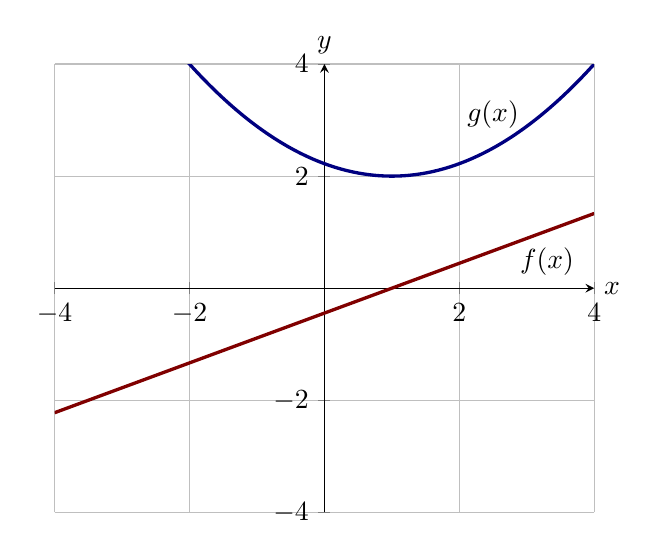
\begin{tikzpicture}
	\begin{axis}
	[ymin=-4,ymax=4, xmin=-4,xmax=4, axis lines=center,xlabel=$x$,ylabel=$y$,every axis y 
	label/.style={at=(current axis.above origin),anchor=south},every axis x label/.style={at=(current axis.right of origin),anchor=west},
	domain=-4:4,
	ytick={-4,-2,2,4},
	yticklabels={$-4$,$-2$,$2$,$4$},
	xtick={-4,-2,2,4},
	xticklabels={$-4$,$-2$,$2$,$4$},
	ymajorgrids=true,
	grid = major
	]
	\addplot[color=penColor, domain=-4:4,very thick,smooth,samples=750]
	{(2/9)*(pow(\x,2)-2*\x+1)+2};
	\addplot[color=penColor2, domain=-4:4,very thick, smooth, samples=250]
	{(4/9)*\x-4/9};
	\node at (axis cs:2.5,3.1) {$g(x)$};
	\node[below] at (axis cs:3.3,0.9) {$f(x)$};
	\end{axis}
       \end{tikzpicture}
\end{center}

One can reasonably infer that the relationship between $g$ and $f$ is given by $\begin{prompt}\answer{g'(x)=f(x)}\end{prompt}$.


\end{exercise}
\end{document}